\section{Results and Analysis}
\label{sec:res}

In this section, we will demonstrate the performance and scalability of our 
selected benchmarks on both host OS and COREMU. These results basically confirms
some of our hypothesis. And finally we're going to see the microbenchmark results. 

First, we'll take a look at the following figures that show the speedup on 
SPLASH-2 and Redis. 
Along the x-axis, we scale the number of processors from 1 to 32. 
The vertical direction shows the speed-up compared to a single-core execution. 

\subsection{SPLASH-2}

Following two figures illustrate the parallelism of SPLASH-2 benchmarks on both QEMU
and native machine. The x-axis indicates the number of cores, which scales from 1
to 32. The y-axis shows the speed-up compared to the performance of one-core
emulation.

\begin{figure}[H]
\center
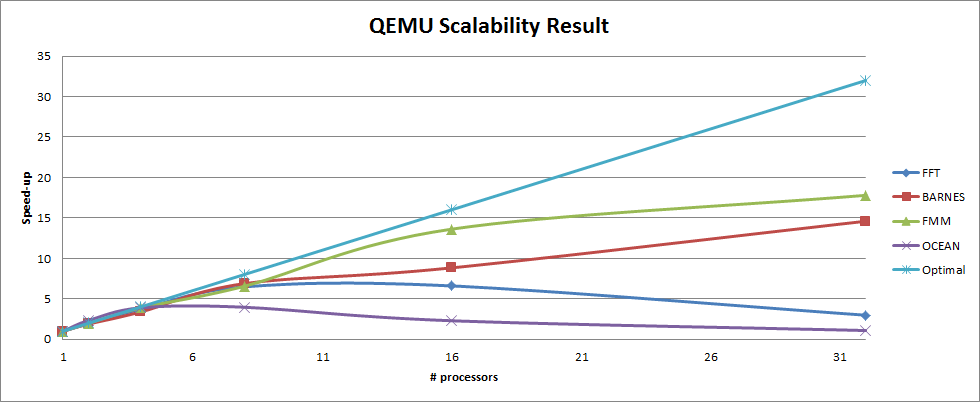
\includegraphics[width=0.8\linewidth]{figures/qm_splash2.png}
\caption{QEMU, splash2}
\label{fig:splash2_vm}
\end{figure}

\begin{figure}[H]
\center
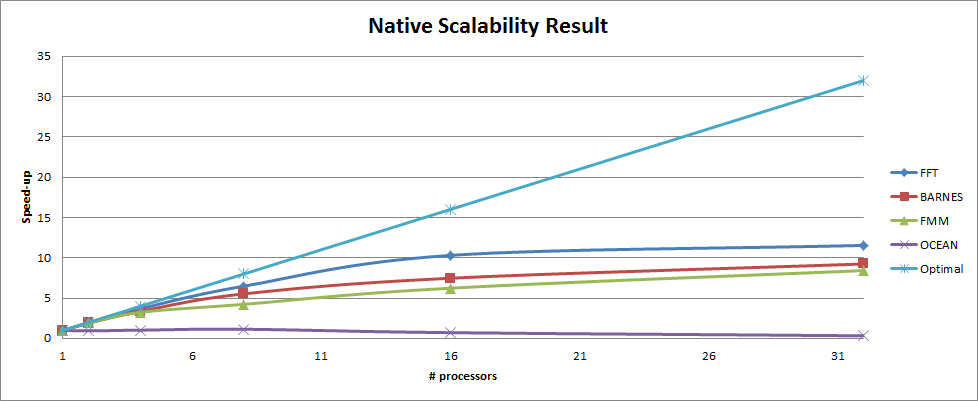
\includegraphics[width=0.8\linewidth]{figures/native_splash2.png}
\caption{Native, splash2}
\label{fig:splash2_native}
\end{figure}

The following table illustrates detailed numbers of the speedup.
\begin{figure}[here]
	\center
	\begin{tabular}{ l | p{2cm} | p{3cm} | p{3cm} | l }
		Benchmark & Number of threads & Speedup in native environment & Speedup in virtual machine & Relative speedup \\
	\hline
FFT & 1 &	1	&	1	&	1	\\
	&	2	&	1.913	&	1.932	&	1.010	\\
	&	4	&	3.683	&	3.711	&	1.007	\\
	&	8	&	6.485	&	6.481	&	0.999	\\
	&	16	&	10.304	&	6.598	&	0.640	\\
	&	32	&	11.538	&	2.976	&	0.257	\\
	\hline
BARNES	&	1	&	1	&	1	&	1	\\
	&	2	&	1.900	&	1.887	&	0.993	\\
	&	4	&	3.361	&	3.376	&	1.004	\\
	&	8	&	5.530	&	6.880	&	1.244	\\
	&	16	&	7.467	&	8.826	&	1.181	\\
	&	32	&	9.237	&	14.593	&	1.579	\\
	\hline
FMM	&	1	&	1	&	1	&	1	\\
	&	2	&	1.923	&	1.980	&	1.030	\\
	&	4	&	3.246	&	3.884	&	1.196	\\
	&	8	&	4.240	&	6.552	&	1.545	\\
	&	16	&	6.240	&	13.613	&	2.181	\\
	&	32	&	8.420	&	17.806	&	2.114	\\
	\hline
OCEAN	&	1	&	1	&	1	&	1	\\
	&	2	&	0.944	&	2.329	&	2.467	\\
	&	4	&	1.027	&	3.891	&	3.788	\\
	&	8	&	1.140	&	3.958	&	3.469	\\
	&	16	&	0.719	&	2.293	&	3.186	\\
	&	32	&	0.333	&	1.076	&	3.223	\\
\end{tabular}
\caption{Relative speedup of the benchmarks}
\label{fig:relspeedup}
\end{figure}

From figures ~\ref{fig:splash2_vm}, ~\ref{fig:splash2_native} and
table ~\ref{fig:relspeedup}, 
we can see that the scalability of the virtual machine system differs from
program to program.

For FFT, it scales better in the native environment. It has speedups 
in the virtualized environment comparable to the native environment up to
8 cores, and then the speedups in the virtualized environment increase
slowly, and with 32 cores the speedup is even lower than the speedup
with 16 cores.

For BARNES, it scales better in the virtualized environment, although the
difference is not very large. The speedup in the virtualized environment
is similar to the speedup in the native environment up to 4 cores, and then
the speedup in the virtualized environment increases slightly faster than
in the native environment, and with 32 cores, the speedup in the virtualized
environment is more than 50 percent larger than the speedup in the native
environment.

For FMM, it scales much better in the virtualized environment. For example, 
when using 32 threads on 32 cores, its speedup relative to using 1 thread 
is more than twice in the virtualized environment than in the native 
environment. Generally, the tread is similar to the BARNES benchmark, where
in this case the speedup in the virtualized environment increases faster.

For OCEAN, it has nearly no scalability in the native environment. The reason
may be that the initialization time is the major part in the execution time,
and the initialization phase may be single-threaded. However, as the number
of cores reaches 16 or 32, its speedup is much lower than 1. This means that there
are some serious scalability problems in OCEAN. Some previous works \cite{rel:oceanscale}
\cite{rel:oceanscale2}
have mentioned these problems, and some have given solutions to some problems.
But in the virtualized environment, it has much better scalability, and
the speedup reaches nearly 4 for 8 cores.

\begin{figure}[here]
	\center
	\begin{tabular}{ l | l | l | l}
	Matrix size &	Number of threads &  Execution time (ns) & Speedup \\
	\hline
	1026 &	1	&	136837351661	&	1\\
	&	2	&	68737401306	&	1.990\\
	&	4	&	34927727140	&	3.917\\
	&	8	&	19920598371	&	6.869\\
	&	16	&	16663947037	&	8.211\\
	&	32	&	19696506618	&	6.947\\
	\hline
	2050 & 	1	&	523716601443	&	1\\
	&	2	&	410726646443	&	1.275\\
	&	4	&	136872166215	&	3.826\\
	&	8	&	67513112087	&	7.757\\
	&	16	&	44456128691	&	11.780\\
	&	32	&	38570262620	&	13.578\\
\end{tabular}
\caption{Speedup of OCEAN with different matrix sizes}
\label{fig:ocean_matrix}
\end{figure}

To further explore the scalability problem of OCEAN, we tried to run the 
benchmark with different matrix sizes. The default sizes is 258x258, and we
guessed that bigger matrix would lead to better scalability, since bigger
matrix usually means that a single thread would have more work to do, and the
communication cost and initialization cost may become a smaller portion in
the total cost. 

In table ~\ref{fig:ocean_matrix}, we showed the benchmark
results with larger matrices, whose dimensions are 1026x1026 and 2050x2050.
From this table, we can see that the scalability increased as expected.
With the matrix of default size, the speedup has its maximum with just 
8 threads.  With a larger matrix with 1026x1026 elements, the maximum speedup
is obtained with 16 threads. With an even larger matrix with 2050x2050
elements, the speedup keeps increasing as the number of threads increases,
and with the maximum number of threads the speedup has its maximum value,
which means that it may further increase with more threads.

\subsection{REDIS}
\begin{figure}[H]
\center
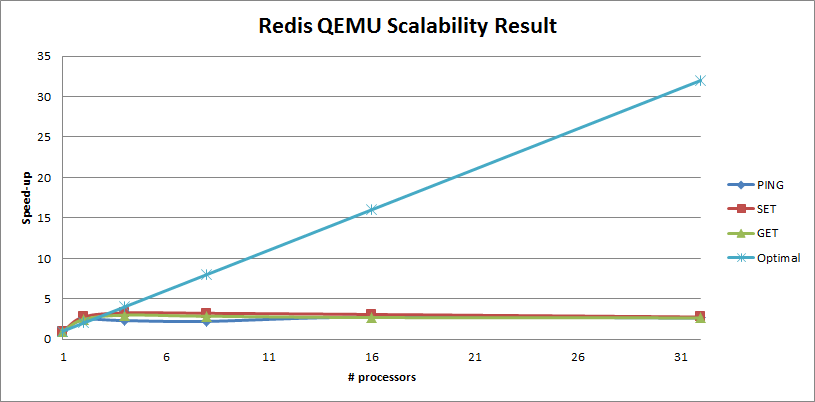
\includegraphics[width=0.8\linewidth]{figures/redis_qemu.png}
\caption{QEMU, REDIS}
\label{fig:redis_vm}
\end{figure}

\begin{figure}[H]
\center
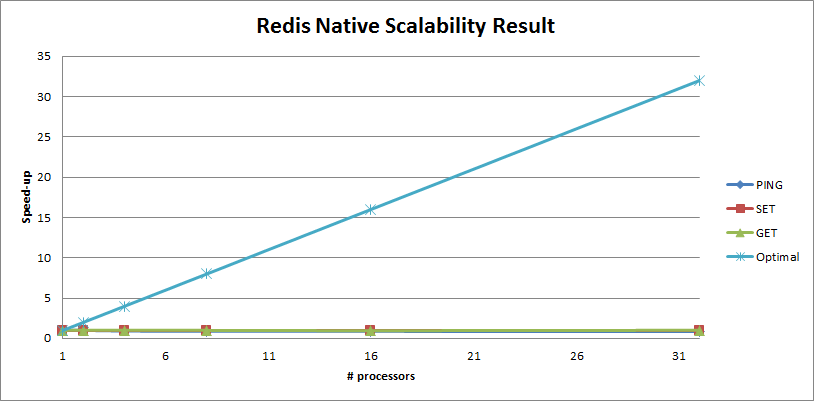
\includegraphics[width=0.8\linewidth]{figures/redis_native.png}
\caption{Native, REDIS}
\label{fig:redis_native}
\end{figure}


From figures ~\ref{fig:redis_vm}, ~\ref{fig:redis_native}, we can see
that REDIS has nearly no scalability in the native environment, and it
only can scale to 2 cores in the virtualized environment. With more than
2 cores, its execution time is nearly constant. It does not run faster
with more cores, and it also does not suffer from more cores. We suspect
that the reason is that the network bandwidth limited the performance
of the REDIS server before the computation resources available from the
CPU become a problem. We partially verified this by looking at the network
bandwidth used and finding that the network usage is nearly full during
the benchmark.


